% !TEX root = ../thesis.tex
%
\chapter{Background and Motivation}%
\label{sec:background}

In this chapter, we are going to introduce the term \emph{Irregular Application}, the concept of \emph{Amorphous Data Parallelism} as well as the parallelism frameworks \emph{Software Transactional Memory} and \emph{Ohua} as a foundation for the following chapters.
We will also briefly discuss the difficulties that arise when reasining about said application types and motivate, why further research into this topic could prove valuable.

\section{Software Transactional Memory}

With the invention of multi-threaded programming, a need for synchronization primitives arose to allow safe parallelization of data-processing applications.
Usually, locks have been used by developers to guard access to pieces of shared data.

Lock-based programming however, has the fundamental drawback of being blocking, meaning that developers have to employ great care when using them in order to not accidentally produce a deadlock (i.e., a state where a number of threads may never again progress) by acquiring locks in the wrong order.
This means a lack of composability, as combining several small lock-based modules into a larger program would require the imposition of some sort of ordering on the locks, which frequently leads to problems.
Even when written correctly, lock-based programs tend to quickly become hard to read and maintain due to the many rules that need to be enforced by the programmer herself without any external checks.

\begin{figure}[h]
    \begin{subfigure}[h]{\textwidth}
    \begin{minted}{Rust}
        let data = TVar::new(12);   // data is a transaction variable
        thread::spawn(move || {
            atomically(|trans| {    // closure for transaction blocks
                let local = data.read(trans)?;
                data.write(trans, local + 2)
            })});
        thread::spawn(move || {
            atomically(|trans| {
                let local = data.read(trans)?;
                data.write(trans, local * 2)
            })});
    \end{minted}
    \caption{Rust code for both transactions.}%
    \label{fig:background:stmcode}
    \end{subfigure}
    \begin{subfigure}[h]{\textwidth}
    \centering
    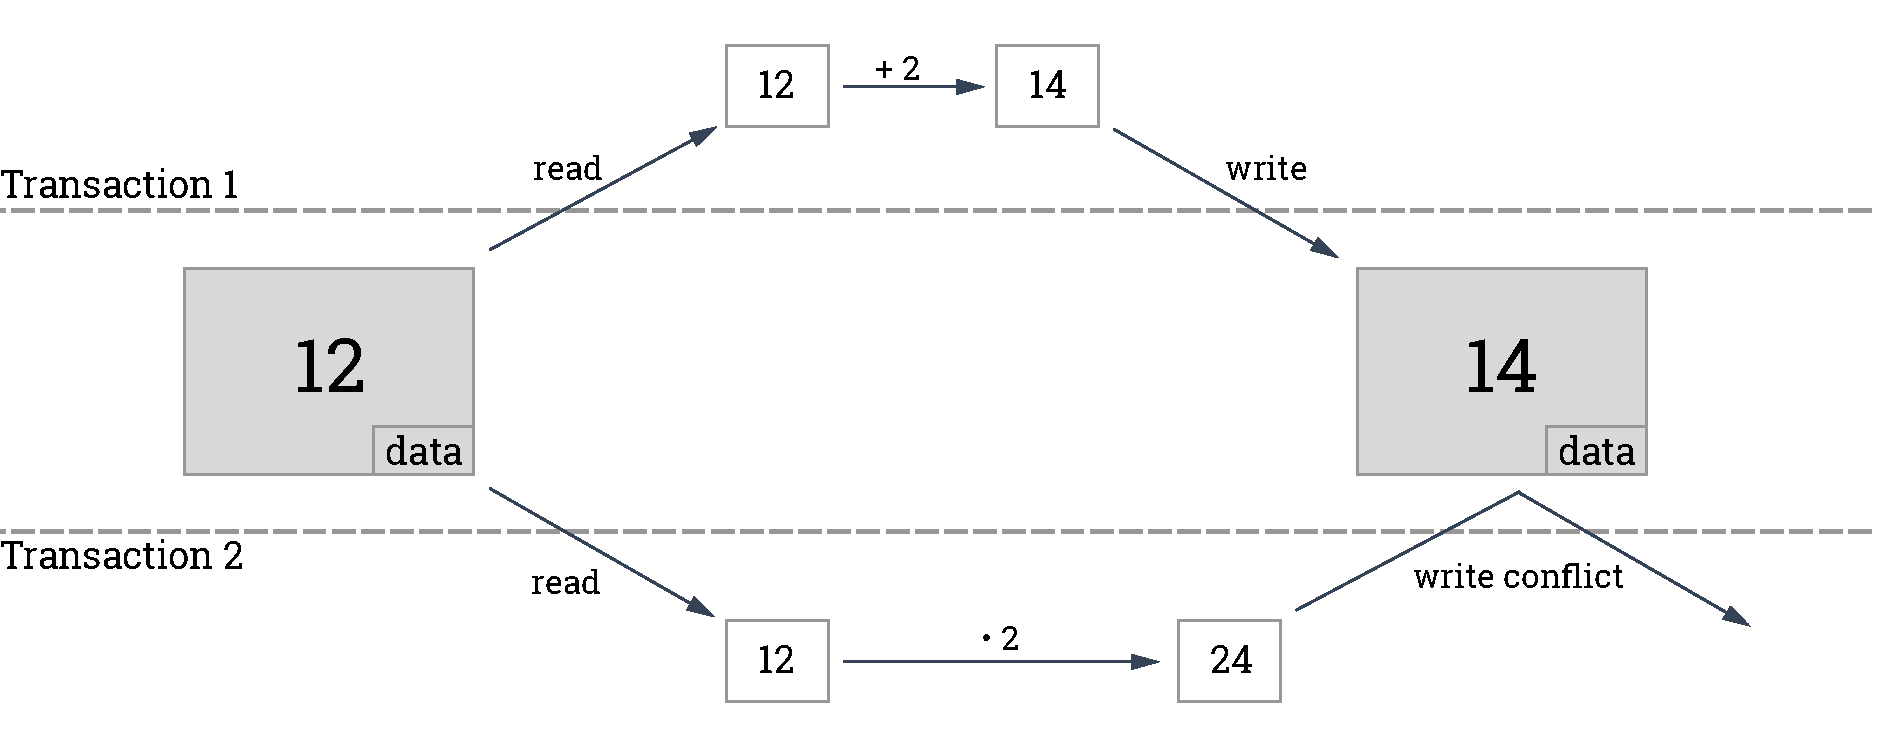
\includegraphics[width=.9\textwidth,keepaspectratio]{gfx/background-stm}
    \caption{Sample execution of two parallel transactions where one transaction has to be rolled back due to a write conflict.}%
    \label{fig:background:stmflow}
    \end{subfigure}
    \caption{Example of two transactions modifying the same shared value in different transactions.}%
    \label{fig:background:stm}
\end{figure}

Hence, Shavit et al.~\cite{shavit1997software} proposed a concept called \emph{Software Transactional Memory}.
This new approach to synchronization aimed to provide lock-free parallelism abstractions that allow multiple threads access to a shared variable without any form of blocking.
Former critical sections are now regarded as \emph{transactions}: They are either executed in their entirety with all their changes taking effect or are not executed at all, just like transactions in databases.
STM's operating principle is outlined in Figure~\ref{fig:background:stm} along with a code example in Fig.~\ref{fig:background:stmcode}.
Every read and write operation to or from a piece of shared data is conducted inside a transaction block and gets initially saved to a local transaction log.
When the transaction block comes to an end, the changes made to individual shared data sections are committed.
Therefore, the changes in the log are applied to the original shared values.
In case another transaction managed to commit in the meantime to a value our transaction also touched, the conflict is detected and instead of committing the changes the transaction is aborted and restarted.
This is normally done until the transaction committed successfully.

In our example in Fig.~\ref{fig:background:stm}, the transactions 1 and 2 both read the same value and modify it.
But since the first transaction was able to commit earlier, the second transaction now stands in conflict and has to be aborted and scheduled for re-execution.

As the example already shows, a fundamental benefit of the (Software) Transactional Memory model is its serializability~\cite{swalens2016transactional}:
All transactions seem to execute serially, since the steps of one transaction never appear to be interleaved with the steps of another transaction.
Therefore, the results of an execution must be equal to the result of a serial execution.
This has been formalized by Swalens et al.~\cite{swalens2016transactional} in their proposed operational semantics for a language with transactions.

Overall, STM takes an optimistic approach to parallelism, because it simply executed numerous computations without any heuristics or reasoning in parallel, hoping for as few conflicts as possible.
The result of this is an underlying non-determinism that ensues everytime transactions are employed in a multi-threaded environment.
Problems in this strategy become apparent when applied to high-contention scenarios.
Since STM may work in parallel over the same data structure or memory region, high contention always leads to a significantly increased number of retries for individual executions, which in turn leads to drastically reduced performance.
Further shortcomings of this concept have been discussed in detail by Caşcaval et al.~\cite{cascaval2008software}.
One the one hand, exception handling becomes impossible to do inside of a transaction without breaking its semantics\todo{Was that what they meant?}.
On the other hand, I/O operations cannot be transactionalized, as well as anything else that producs side effects outside of te transactions scope as these effects may not be rolled back on error.
Additionally, they reported large overheads of STM applications for smaller worksets as well as no debuggability, since the non-determinism makes certain situations nearly irreproducable.

\section{Irregular Applications}

In the past, most of the research conducted in the field of performance improvements for parallel programs has concerned itself with what is called regular applications.
There are applications, whose degree of exploitable parallelism is simply determined by the program structure and the size of the input set.
As both of there properties are known or can be inferred at compile time, any optimization potential is easy to uncover and exploit for compilers.

When looking at \emph{irregular applications} on the other hand, the situation is completely different.
The term describes applications, whose structure resolves around the manipulation of large, pointer-based data structures like graphs and trees.
Due to this structural peculiarity, compiler analyses struggle to uncover any meaningful insights into the algorithm that would allow to exploit any parallelism hidden in it.

\begin{figure}[b]
    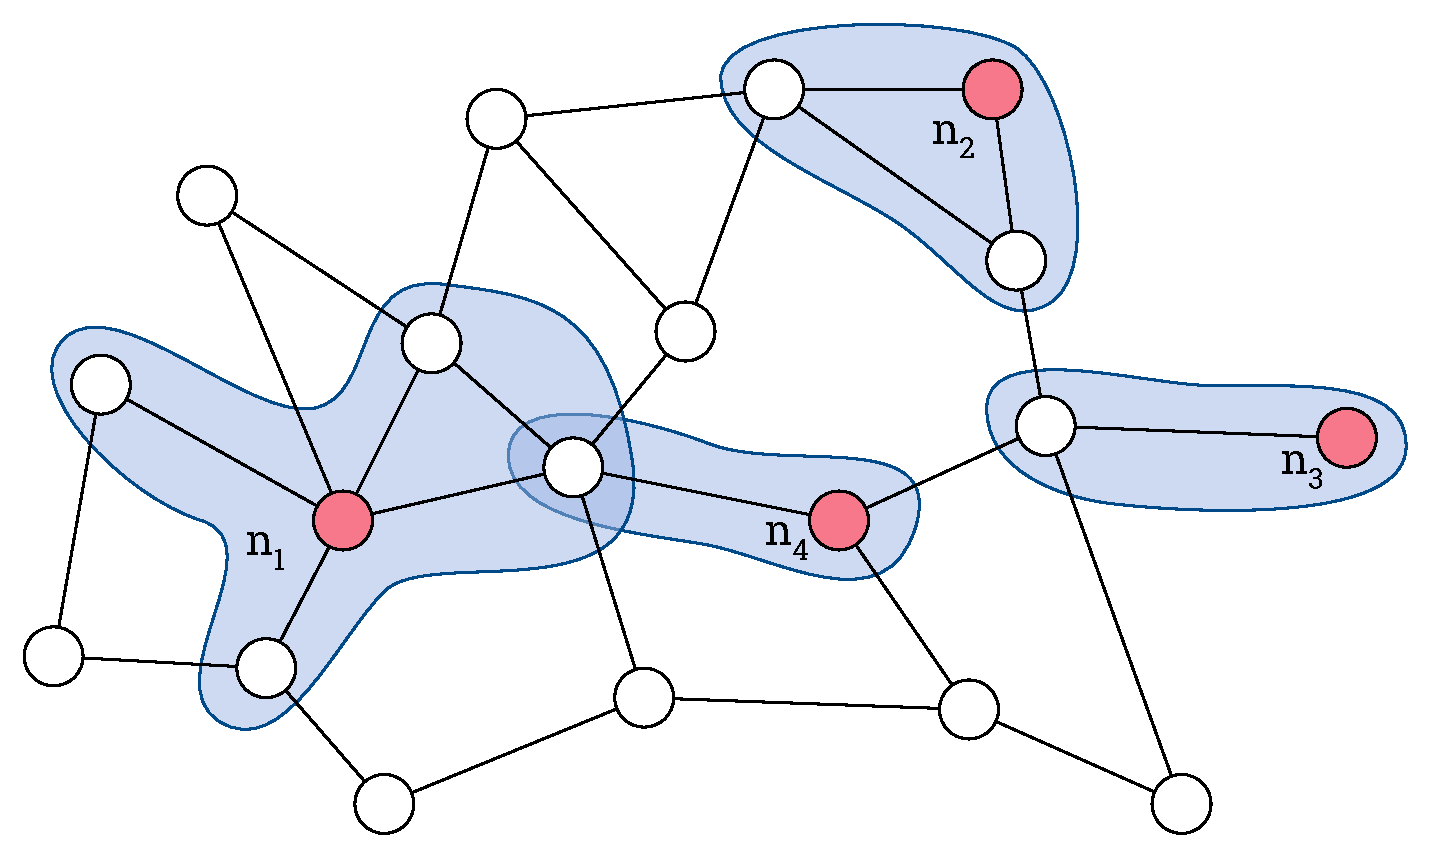
\includegraphics[width=.7\textwidth,keepaspectratio]{gfx/background-irregular}
    \caption{Graph representation of an irregular application with active elements and their neighborhoods. Adapted from Kulkarni et al.~\cite{kulkarni2009much}}%
    \label{fig:background:irregular}
\end{figure}

To better outline this, Kulkarni et al.~\cite{kulkarni2009much} developed an abstract representation for irregular programs using a set of nodes and edges, as shown in Fig.~\ref{fig:background:irregular}.
The nodes and edges represent the input data and their relationships.
During the execution of an irregular algorithm, the program may perform computations on a (sub-)set of active nodes or edges, the work items.
In Figure~\ref{fig:background:irregular}, these are highlighted in red.
Performing said executions may involve reading from or writing to other nodes or edges in the graph, which form an active elements' neighborhood, shaded in blue.
Which elements of the graph make up the neighborhood of an active element is not known beforehand and may encompass all direct neighbors in the graph (as seen for nodes $n_2$ and $n_3$), maybe only a single neighboring element (as seen for node $n_4$) or transitively the neighboring elements of its direct neighbors.

Usually, work items are not ordered and may be processed in any order.
But processing one element may generate an arbitrary number of new active elements or remove others from the pool, depending on the algorithm.
Also, some active elements may not be processed simultaneously due to overlapping neighborhoods, as the changes made by processing both items may conflict with each other.

Since all these relationships and interdependencies are not known beforehand but rather depend on the input data, this information cannot be uncovered and used by compile time analyses.
And because static parallelization as well as lock-based approaches fail\todo{isn't that too harsh for locking?} to uncover any parallelism opportunities in these programs, Kulkarni et al.~\cite{kulkarni2007optimistic} argue, that optimistic strategies such as \emph{Software Transactional Memory} need to be used to tackle this class of problems.
This is because, as we have shown, the heavy use of pointers in the program hinders efficient analyses but as conflicts due to parallelization may be rare (depending on the input data) the optimistic trial-and-abort semanticsof STM allow for a simple and efficient parallelization in most cases.


\subsection{Amorphous Data Parallelism}

Pingali et al.~\cite{pingali2009amorphous} argue, that most irregular applications additionally exhibit a behavior referred to as \emph{amorphous data parallelism}:

Given a set of active nodes and an ordering on them, amorphous data parallelism is the parallelism that arises from simultaneously processing active nodes and is subject to neighborhood and ordering constraints.
It is a generalization of standard data parallelism in which
\begin{enumerate}
    \item concurrent operations may conflict with each other
    \item activities can be created dynamically
    \item activities may modify the underlying data structure
\end{enumerate}
These characteristics have already been briefly discussed in connection with Fig.~\ref{fig:background:irregular}.

While irregular applications are hard to readon about due to their pointer usage, they are still a very interesting research topic, made more difficult by amorphous data parallelism.
But as we will show in chapter~\ref{sec:experiments}, applications of this type are common and widespread in different aspects of real world applications.



\section{Ohua}



% - present both Ohua and STM
%   - explain paradigms in detail (most people here don't know what stm is and how it works!)
%   - detail benefits and shortcomings of both
%   - Ohua: talk about the compiler, its stages and where optimizations hook in as this will be required information later on.
%   - STM: Detail that non-determinism is part of the execution model -> speculative parallelism
%       - make sure to thoroughly explain the concept of a transaction
%   - Ohua: detail determinism of the model if appropriate, but remember that this will also be discussed later on
% - explain Irregular Applications: They are different from the parallelizability problems we usually face as the input dictates the parallelism at runtime and the computing times!
%   - use: \label{sec:background:irregular}
